\documentclass[oneside]{amsart}
\usepackage{amsmath}
\usepackage{amsfonts}
\usepackage{amsthm}
\usepackage{hyperref}
\usepackage{amscd}
\usepackage{color}
\usepackage{enumerate}
\usepackage{xypic}
\usepackage{tikz}


\newcommand{\cond}{\mathbf{Z}}
\newcommand{\bl}{\boldsymbol{\ell}}
\newcommand{\A}{\mathcal{A}}
\newcommand{\ZZ}{\mathbb{Z}}
\newcommand{\KK}{\mathbb{K}}
\newcommand{\RR}{\mathbb{R}}
\newcommand{\PP}{\mathbb{P}}
\newcommand{\CC}{\mathbb{C}}
\newcommand{\QQ}{\mathbb{Q}}
\newcommand{\NN}{\mathbb{N}}
\newcommand{\HOT}{(\star\star\star)}

\DeclareMathOperator{\trop}{Trop}
\DeclareMathOperator{\vol}{Vol}
\DeclareMathOperator{\conv}{conv}

\newtheorem*{mainthm}{Main Theorem}
\newtheorem{thm}{Theorem}[section]
\newtheorem{prop}[thm]{Proposition}
\newtheorem{lemma}[thm]{Lemma}
\newtheorem{cor}[thm]{Corollary}
\newtheorem{claim}[thm]{Claim}
\newtheorem{fact}[thm]{Fact}
\newtheorem{example}[thm]{Example}
\newtheorem{conj}[thm]{Conjecture}

\newtheorem{lem}[thm]{Lemma}
\theoremstyle{definition}

\newtheorem{defn}[thm]{Definition}

\newtheorem{definition}[thm]{Definition}
\newtheorem{rem}[thm]{Remark}
\newtheorem{question}[thm]{Question}
\newtheorem{ex}[thm]{Example}

\newcommand{\nathan}[1]{\textcolor{red}{#1}}
\newcommand{\yoav}[1]{\textcolor{blue}{#1}}
\newcommand{\bernd}[1]{\textcolor{green!60!black}{#1}}
\newcommand{\kristin}[1]{\textcolor{purple}{#1}}

\title{Tropical Dual Curves}

\author{Nathan Ilten}
\address{Department of Mathematics, Simon Fraser University,
8888 University Drive, Burnaby BC V5A1S6, Canada}
\email{nilten@sfu.ca}

\author{Yoav Len}
\author{Bernd Schober}
\author{Kristin Shaw}
\begin{document}

\begin{abstract}
Abstract to come. Now there's an abstract
\end{abstract}
\maketitle
\section{Preliminary Notes}
A smooth tropical plane curve $C\subset \mathbb{R}^2$ is dual to a primitive
subdivision of its Newton polygon. We will also assume that  two edges  of $C$
are contained in a line  \kristin{Don't understand this assumption. This was to
avoid certain non-lifting bitangents right?
Still think there is a typo here} \yoav{Yes, I think that condition was only relevant for bitangents.} For $v\in\RR^2$, let
$L_v$ denote the tropical line with vertex $v$.

\begin{defn}
A \emph{tropical tangent} of a smooth tropical plane curve $C$ is a tropical line $L_v$ satisfying one of the following:
\begin{enumerate}
\item \label{item:deg2} $L_v$ intersects an edge $E$ of non-transversely and compactly;
\item $L_v$ intersects $C$ transversely at a vertex $w$ of $C$. \label{item:tan2}
\item $L_v$ intersects $C$ transversely at the vertex $v$; or \label{item:tan3}
\end{enumerate}
\end{defn}

The \emph{tropical dual curve} $C^*$ of $C$ is the weighted polyhedral complex consisting of all $v\in\RR^2$ such that $L_{-v}$ is a tropical tangent of $C$, where we attach weight $2$ to all tangents of the form \ref{item:deg2}.

For a tropical curve $C$, we can describe $C^*$ a bit more explicitly.
\begin{itemize}
\item For any vertex $w$ of $C$, and any edge direction $u$ emanating from $w$ such that $-u$ is the edge direction of a tropical line, $C^*$ has an unbounded weight two edge emanating from $-w$ in direction $-u$. This covers all tropical tangents of type \ref{item:deg2}. 
\item For any vertex $w$ of $C$, and any edge direction $u$ of a tropical line not parallel to an edge of $w$, $C^*$ has an unbounded weight one edge emanating from $-w$ in direction $u$. This covers all tropical tangents of type \ref{item:tan2}.
\item For any vertex $w$ of $C$, and any edge direction $u$ emanating from $w$ not parallel to a tropical line, $C^*$ has a weight one edge emanating from $-w$ in direction $-u$. The length of the edge is exactly the length of the corresponding edge of $C$. This covers all tropical tangents of type \ref{item:tan3}.
\end{itemize}
\begin{lemma}
The weighted polyhedral complex $C^*$ satisfies the balancing condition.
\end{lemma}
\begin{proof}
%\nathan{This will follow from the fact that $C^*$ is the tropicalization of a dual curve, but we should show that we can see this without using that fact. This should be an easy local check.}
\bernd{Let $ w^* $ be a vertex of $ C^* $ and 
let $ w $ be the corresponding vertex of $ C $, $ w^* = - w $.
Let $ v_1, \ldots, v_d $ be the primitive vectors determining the edge directions emanating form $ w $ and 
which are not parallel to an edge of a tropical line.
Let $ u_1, u_2, u_3 $
%$ u_1 := -e_1, u_2 := -e_2 $, and $ u_3 := e_1 + e_2 $ 
be the edge directions of a tropical line.
Since all edges of $ C $ have weight one,
the balancing condition at $ w $ states
\begin{equation}
\label{eq:bal_C}
	\sum_{i=1}^d v_i + \sum_{j=1}^3 (a_j u_j + b_j (-u_j)) ) = 0,
\end{equation}
for certain $ a_j, b_j \in \{ 0 ,1 \} $.
By the construction of $ C^* $, we need to show
$$
	\sum_{i=1}^d (-v_i) + \sum_{j=1}^3 2b_j u_j + \sum_{j=1}^3 (1-a_j)(1-b_j) u_j \stackrel{!}{=} 0
$$
in order to get that $ C^* $ is balanced at $ w^* $.
% \sum_{i=1}^d (-v_i)  tropical tangents of type \ref{item:tan3}
% \sum_{j=1}^3 2b_j u_j   tropcial tanagents of type \ref{item:deg2}
% \sum_{j=1}^3 (1-a_j)(1-b_j) u_j  tropical tanges of typoe \ref{item:tan2}
Using \eqref{eq:bal_C} and the fact $ u_1 + u_2 + u_3 = 0 $, 
the left hand side becomes $ a_1 b_1 u_1 + a_2 b_2 u_2 + a_3 b_3 u_3 = 0 $.
Since no two edges of $ C $ are contained in a single line, we have $ a_j b_j = 0 $, for all $ j \in \{ 1,2,3\} $.
Thus the balancing condition holds a $ w^* $ and this implies the assertion.}
\end{proof}


\begin{proof}
\kristin{	
Let $w^*$ be a vertex of $C^*$. First notice that there must be a vertex $w$ dual to 
$w^*$. By the assumptions that $C$ be a non-singular tropical curve the vertex $w$ is 
trivalent. Let $v_1, v_2, v_3$ denote the three \emph{outgoing} primitive integer 
vectors parallel to the three edges of $C$ adjacent to $w$.\\ 
%
If the set  $V:= \{v_1, v_2, v_3\}$ is disjoint from  $$E:= \{\pm(-1, 0),
\pm(0, -1), \pm(1, 1)\}, $$ then all edges adjacent to $w^*$ come from tropical
tangents of type $(2)$ and type $(3)$.
Therefore, all edges of $C^*$ adjacent to $w^*$ are of weight $1$ and the set of their 
primitive integer directions are precisely, 
$$\{v_1, v_2, v_3, (-1, 0), (0, -1), (1, 1)\}.$$
Therefore, the dual curve $C^*$ is balanced at $w^*$ by the balancing of $C$ at $w$.\\  
%
By the balancing condition on $V$, the set $|V \cap E| = 1$ or $3$.  If $|V \cap E| =
3$ then $V = \{(-1, 0), (0,-1) (1, 1)\} $ or $\{(1, 0), (0, 1) ,(-1, -1)\}$. In
both cases, all edges of $C^*$ adjacent to $w^*$ are due to tangents of  type
$(1)$. In partcular, the edges of $w^*$ are all of weight $2$. In the first case it is easy to check that for every bounded edge of $C$ adjacent to $w$ in direction $v$ there are
$2$ edges of $C^*$ adjacent to $w^*$ in directions $\pm v$, with each edge
being of weight $2$. So that the dual curve is clearly balanced at $w^*$. In
the second case, there are three  edges adjacent to $w^*$, each of weight $2$
and in directions $\{(-1, 0), (0, -1), (1, 1)\}.$ \\
%
Now, consider the case when $|V \cap E| = 1$ and without loss of generality
suppose $v_1 = E \cap V$. If either, $v_1 \in \{- (1, 0), -(0, 1), -(1, 1)\}$ or
the edge in direction of $v_1$ is bounded then there are two edges of  weight $2$ 
adjacent to $w^*$ in directions $\pm v_1$. Let $e_2$ and $e_3$ denote the edges of $C$
adjacent to $w$ in directions 
$v_2,$ and $ v_3$, respectively. Then we get tangents of type $(3)$ along the edges $e_1$
and $e_3$ giving edges of $C^*$ adjacent to $w^*$ in directions $-v_2$, $v_3$. Also we get
tangents of type $(2)$ to $C$ by moving $L_w$ in directions $(0, -1)$ and $(1, 1)$. These give edges of $C^*$ adjacent to $w^*$ in directions $(0, 1)$ and $(-1, -1) $. 
Now it is easy to check that $C^*$ is balanced at $w^*$.\\
%
Lastly if  $v_1 \in \{ (-1, 0), (0, -1), (1, 1)  \}$ and the 
edge of $C$ in direction $v_1$ is unbounded. Then it is a straight forward check that 
there are $4$ edges adjacent to $w^*$ and their directions are $-v_2, -v_3$ and $(0, -1), (1, 1)$. Therefore, $C^*$ is balanced at $w^*$.   
}
\end{proof}

\begin{conj}
Given the dual curve $C^*$ we can recover $C$ under some assumptions. 
\end{conj}

\kristin{\textbf{Ok, I realise that anything is true under the right
assumptions but I really think there is something non-trivial here :) Also we
should take a look at the paper about tropical inflection points, it should
give us a hint about cuspidal points on the dual curve. This would complement
Yoav's work with Hannah.}}

Let $X=V(f)\subset \PP^2$ be an irreducible plane curve. If $X$ is sufficiently generic with respect to its Newton polytope, then $\trop(X)$ satisfies the assumptions imposed on $C$ above.

\section{Lifting tropical tangents}



Let  $\mathcal{L}_0, \mathcal{L}_1, \mathcal{L}_2$ be lines in $\mathbb{K}P^2$ such that  $\mathcal{L}_0 \cap \mathcal{L}_1 \cap \mathcal{L}_2 = \emptyset$. Set $\mathcal{D} = \cup_{i = 0}^2 \mathcal{L}_i$

This section is devoted to proving the lemma. 

\begin{defn}
Let $C  = \text{Trop}(X \cap (\KK^*) \subset \mathbb{R}^2$ be a tropical curve. A tropical line $L \subset \mathbb{R}^2$  \textit{lifts to a  tangent of $X$} if there exists 
a line $\mathcal{L} \subset \mathbb{K}P^2$ such that $\mathcal{L}$ is tangent to $\mathcal{C}$ and  $\text{Trop}(\mathcal{L}) = L$. 

%Let $x \in \mathbb{R}^2$, and $L$ a tropical line. Then $L$ is a \textit{liftable tangent at $x$} if $L$ is a liftable tangent and 
\end{defn}

\begin{prop}\label{prop:lifting}
Every tangent line of $X$ meeting $(\KK^*)^2$ tropicalizes to a tropical tangent of $\trop(X)$. Conversely, every tropical tangent of $\trop(X)$ lifts to a tangent line of $X$. Tropical tangents of type \ref{item:deg2} lift to two distinct $1$-parameter families of tangents, whereas tropical tangents of the other types lift to a single family. \nathan{Make this more precise}.
\end{prop}


A key tool in classifying tropical lines which lift to tangent lines of a curve $X$ is the tropical stable intersection. Given two tropical curves $C_1$ and $C_2$ their tropical stable intersection $C_1 \cdot C_2$  is supported on the zero skeleton of the set theoretic intersection of $C_1$ and $C_2$, namely $(C_1 \cap C_2)^{(0)}$. The multiplicity of a point  $x \in (C_1 \cap C_2)^{(0)}$
is 
$$m_x( C_1 \cap C_2) := \text{MV}( \Delta_1(x), \Delta_2(x)),$$
where $\Delta_i(x)$ is the polytope dual to the point $x$ in the dual subdivision of the curve $C_i$ and $\text{MV}$ denotes the mixed volume. 

For a connected component $E$ of $C_1 \cap C_2$ define
$$m_E(C_1 \cdot C_2) := \sum_{x \in (C_1 \cap C_2)^{(0)}} m_x( C_1 \cdot C_2). $$
\begin{lemma}\label{lemma:stableint}
Let $C   = \text{Trop}(X) \subset \RR^2$ be a tropical curve and $L \subset \RR^2$ a tropical line. If $L$ lifts to a tangent line of $X$ then there must be a connected component $E$ of $C \cap L$ such that $m_E( C \cdot L) \geq 2$. 
\end{lemma}

\begin{proof}
This lemma is a special case of Proposition 3.11 from \cite{BrugalleLopez}. 
\end{proof}


In fact, a variant of this approach to determining the tropicalization of tangent lines  was used to determine the tropicalization of inflection points and their tangent lines in \cite{BrugalleLopez}. There the authors were searching for lines $L$ and connected components $E$ such that  $m_E(C \cdot L) \geq 3$. 


Let $\{f=0\}$ be a curve in $\mathbb{P}^2$. For a line $\{\ell=0\}$ is tangent to $f$ at a point $p$, it is necessary and sufficient that  that $f(p)=\ell(p)=W(p) = 0$, where $W$ is the Wronskian 
\[
f_x\ell_y - f_y\ell_x.
\] 

Now, suppose that $\Lambda$ is a tropical line, tangent to $\Gamma=\trop(f)$ at a point $q$. We will find coefficients $m,n,k\in K$ and a point $p\in\mathbb{R}^2$ so that the line $\ell= (y+m+nx)$ tropicalizes to $\Lambda$, the point  $p$ tropicalizes to $q$, and the functions $f,\ell,W$ vanish at $p$. Moreover, we will show that there is a finite number of $1$-parameter families satisfying these conditions. 

The strategy is as follows. First, we compute the leading terms of the coefficients. Then, we find expressions for the next order terms. Finally, we show that the leading terms can be extended to Puiseux series, using the non-Archimedean implicit functions theorem. We will deal with each combinatorial type of  intersection separately. We begin with a concrete example. 

\begin{example}\label{ex:properIntersection}
Let $f = x+y+x^2+O(t)$, denote $\Gamma = \trop(f)$, and let $\Lambda$ be a tropical tangent to $\Gamma$ at the origin, as in Figure \ref{ProperHorizontal}. Let $(k,0)$ be the vertex of $\Lambda$. We need to find $\ell = y+m+t^kn$ with  trivially valued $m$ and $n$ that is tangent to $f$ at a point with trivially valued coordinates. 

The Wronskian in this case is $W= f_x\ell_y - f_y\ell_x = 1+2x+ O(t)$. While the terms hidden in the $O(t)$ part effect the solution of the computation below, they only contribute constant terms, and the number of lifts of the tangent will not depend on them. Let $(x,y) = (x_0+tx', y_0+ty')$ be a point tropicalizing to $(0,0)$. 

Considering the valuation 0 part of $\ell,q,W$, we see that 

\begin{gather*}
y_0 + m_0 = 0,\\
x_0+y_0 + x_0^2 = 0,\\
1+2x_0 = 0.
\end{gather*}
Solving the system we get
\[x_0 = -\frac{1}{2}, y_0 = \frac{1}{4}, m_0 = -\frac{1}{4}. \]

Next, we write expressions for $x',y',m'$ by considering the terms with valuation $1$. If $k=1$ then $\ell$ yields $y'+m'+n_0 = O(t)$, and if $k>1$ then $y'+m'=O(t)$. In either case,  
\begin{equation}\label{eqLine}
y'+m'=C_1+O(t),
\end{equation}
where $C_1$ is a constant that does not depend on $x',y',m'$.  
From $f$ we have 
$x' + y' + 2x_0x' = C_2 +  O(t)$, where again, $C_2$ is a constant. Since we already know that $x_0 = -\frac{1}{2}$, we get 
\begin{equation}\label{eqCurve}
y' = C_2 + O(t).
\end{equation}
Finally, from $W$ we have  
\begin{equation}\label{eqWronskian}
2x' = C_3.
\end{equation}

Let $g_1,g_2,g_3$ be the left hand side of Equations \ref{eqLine},\ref{eqCurve},\ref{eqWronskian}. Then by the implicit function theorem, we can find Puiseux series $x',y',m'$ satisfying the equations if  the matrix of partial derivates
\[
\begin{pmatrix}
  \frac{dg_1}{dx'} & \frac{dg_1}{dy'} & \frac{dg_1}{dm'} \\
  \frac{dg_2}{dx'} & \frac{dg_2}{dy'} & \frac{dg_3}{dm'} \\
  \frac{dg_3}{dx'} & \frac{dg_3}{dy'} & \frac{dg_3}{dm'}
 \end{pmatrix} 
 \]
 is non-singular. And indeed, its determinant is 
\[
\det\begin{pmatrix}
  0 & 1 & 1 \\
  0 & 1 & 0 \\
  2 & 0 & 0
 \end{pmatrix} = 2 \neq 0.
 \]
The computation above did not depend on the choice of $n$, so for any choice of $n$ with valuation zero, there is a unique line $\ell$ lifting $\Lambda$. 


\begin{figure}
\centering
\begin{tikzpicture}[scale=.5]

\draw[thick, blue] (0,0) to (-5,0);
\draw[thick, blue] (0,0) to (0,-3);
\draw[thick, blue] (0,0) to (3,3);
\node [right] at (2,2) {$\Lambda$};
{\tiny \node [right] at (0,0) {$(k,0)$};}

\draw[purple] (-2,0) to (-1,2);
\draw[purple, dotted] (-1,2) to (-0.8,2.4);
\draw[purple] (-2,0) to (-2,-1);
\draw[purple, dotted] (-2,-1) to (-2,-1.2);
\draw[purple] (-2,0) to (-3,-1);
\draw[purple, dotted] (-3,-1) to (-3.2,-1.2);
\draw[fill,purple] (-2,0) circle [radius=0.08];

\node [right] at (-1,2) {$\Gamma$};

\end{tikzpicture}   

\caption{Proper intersection along a horizontal edge}
\label{ProperHorizontal}
\end{figure}


\end{example}


The following trick which can be easily verified will be useful for simplifying the step of equating coeffificents with valuation $1$. 
\begin{fact}\label{fact:trick}
Let polynomial $g\in K[x,y]$, and suppose that $g(x_0 + x't,y_0+y't) = 0$. Then $g_x\cdot x' + g_y\cdot y' = C + O(t)$, where $C$ is a constant that does not depend on $x',y'$.  
\end{fact}

\subsection{Transverse intersection at the interior of two edges}
Suppose that $\Lambda$ and $\Gamma$ meet transversally with multiplicity at least $2$ at a point $q$ in the interior of edges of both of them. 
Then  $\Lambda$ does not lift to a line $\ell$ that is tangent to $f$, by \cite[Lemma 3.13]{BrugalleLopez}.  

To see this using the approach of the Wronskian, let $q$ be the tropical point of intersection, and assume that it is at the origin. Without loss of generality, we  may assume that $q$ it is at a horizontal edge of $\Lambda$. Write $\ell = y+m+nx$ for some trivially valued $m$, and a positively valued $n$, and $f = ax^i + by^j + O(t)$ for some $a,b,i,j$. It follows that the Wronskian of the system is $W = iax^{i-1} + O(t)$, which never vanishes for trivially valued $x$, a contradiction. 

%\subsection{Intersection at a vertex of the line and an edge of the curve} 
\subsection{\kristin{Intersection at an edge of the line and a vertex of the curve}}\label{sec:edgelinevertcurve}
This is a generalization of Example \ref{ex:properIntersection} above.
Suppose that the edge of $\Lambda$ intersects the vertex $q$ of the curve $\Gamma$ and let $E$ be the connected component of $\Gamma \cap \Lambda$ containing the vertex $q$. 
In order for $\Lambda$ to lift to a tangent, by Lemma \ref{lemma:stableint} we must have $m_E(\Gamma \cdot \Lambda) \geq 2$. We claim that unless $\Lambda$ is a tropical tangent of type $(1)$, we must have that $E = q$. If $E \neq q$ then  $\Lambda $ and $\Gamma$ must intersect along an edge adjacent to the vertex $q$, if this edge is unbounded then $q = 
E \cap (\Gamma \cap \Lambda)^{(0)}$ so that $m_q(\Gamma \cap \Lambda) = \text{MV}(\Delta_{\Gamma}(q), \Delta_{\Lambda}(q)  \geq 2$. But this is impossible since $\Delta_{\Gamma}(q)$ is unimodular and $\Delta_{\Lambda}(q)$ is an edge of $\Gamma$. 
Therefore, if $\Lambda$ is liftable to a tangent (not of type $1$), then $\Lambda$ and $\Gamma$ must intersect transversally at $q$. 

We now show that all such tropical lines lift to tangents. Assume without loss of generality that $q = (0, 0)$ is contained in the  horizontal edge of the line and that the vertex of $\Lambda$ is at $(k,0)$ for some $k\in\mathbb{Z}$. Then $\ell = y+m+t^knx$, where $m = m_0 + tm'$ for some $m_0\in\mathbb{C}$ and $m',n$ with trivial valuation. %\kristin{I guess we are using -val for tropicalization not val?}
\kristin{\textbf{$k$ is used twice here for different things}}
Write
\[
f = a+ bx^iy^j + cx^ky^l + O(t).
\]
Then the Wronskian is 
\[
W = f_x  + O(t) = ibx^{i-1}y^j + ckx^{k-1}y^l + O(t).
\]

Let 
$p=(x,y)$
 where $\kristin{x} = x_0 + x't,  \kristin{y} = y_0+y't$ for $x',y'$ with trivial zero.
We begin by finding the leading coefficients $x_0,y_0$. From $W$ we get $x_0^iy_0^j = \frac{c_0kx_0^ky_0^{l}}{ib_0}$. Plugging this into $f$ we get $x_0^ky_0^{l} = B$ and $x_0^iy_0^j = A$, for constants $A,B$ that only depend on $a,b,c$. Since $\Gamma$ is smooth, the vectors $(i,j)$ and $(k,l)$ form a unimodular basis, and so we can find $\mu_1,\nu_1$ and $\mu_2,\nu_2$ such that $\mu_1 (i,j) + \nu_1 (k,l) = (1,0)$ and $\mu_2 (i,j) + \nu_2 (k,l) = (0,1)$. It follows that 
\[
x_0 = \frac{(x_0^i y_0^j)^{\mu_1}}{(x_0^k y_0^{l})^{\nu_1}} = \frac{A^{\mu_1}}{B^{\nu_1}},
\]
and 
\[
y_0 = \frac{(x_0^i y_0^j)^{\mu_2}}{(x_0^k y_0^{l})^{\nu_2}} = \frac{A^{\mu_2}}{B^{\nu_2}}.
\]

Next, we find expressions for $x',y',m'$, and use the non-Archimedean implicit function theorem to show that there exist unique Puiseux series satisfying these relations. Using \ref{fact:trick} for  $\ell, f, W$ we compute 
\[
y'+m' + C_1 = O(t),
\]

\[
f_x(x_0,y_0)\cdot x' + f_y(x_0,y_0)\cdot y' + C_2 = O(t),
\]
and 
\[
f_{xx}\cdot x' + C_3 = O(t).
\]
Note that we already know that $f_x(x_0,y_0) = 0$.
To use the  implicit function theorem, we need to show that the determinant of the Jacobian doesn't vanish. Indeed, 
\[
\det\begin{pmatrix}
  0 & 1 & 1 \\
  0 & f_y(x_0,y_0) & 0 \\
  f_xx(x_0,y_0) & f_xy(x_0,y_0) & 0
 \end{pmatrix} = a_0\cdot k\cdot y.
 \]
The fact that the intersection multiplicity at $q$ is greater than $1$ implies that $k,i\neq 0$. The computation did not depend on the value of $n$, and therefore the tangent lifts uniquely for any choice of trivially valued $n$.

\subsection{Intersection at an edge of the curve and a vertex of the line} 

A similar argument to the beginning of Subsection \ref{sec:edgelinevertcurve} shows that if  a line intersecting an edge of a curve at its vertex $q$ is liftable to a tangent line then the line and curve must intersect transversely at the vertex. 

\kristin{I would like to use the following trick so as not to repeat the long calculation again. Consider a linear transformation $\text{GL}_2(\ZZ)$ sending the edge of the curve to the horizontal direction. Then the image of the tropical line becomes a curve. We want to show that if the coefficients of one or the other are fixed we can find coefficients of the other so that the two curves have a point of multiplicity two in the preimage of the vertex, hence a tropical tangent. } 
%Now assume that the vertex of the tropical  line $\Lambda$ is at $(0, 0)$ so that it is the tropicalization of a line defined by:
%$\ell = y+m+nx$, with $m$ and $n$ having trivial valuations. The equation for a lift of the curve $\Gamma$ is then 
%\[
%f = a+ bx^iy^j + O(t^{v+1}), 
%\]
%with the valuations of  $a$ and $b$ being equal to $v$. 
%Let the equation of the line be once again  $\ell = y+m+nx$, with $m, n$ having possibly non-trivial valuations. 
%$i) val(m) = 0 $ and $val(n) >0$. 
%$ii) $
%$ii)   $. 
%The Wronskian then becomes: 
%\[
%W = f_x  +  f_y\ell_x = ibx^{i-1}y^j +  jbnx^{i+1}y^{j-1} + O(t).
%\]


%This determines which edge of the tropical line passes through the vertex $(0, 0)$ of the curve $\Gamma$. 

\subsection{Intersection is a compact edge} 
\begin{example}
Let $\Gamma$ be the tropicalization of 
\[
f = x+xy+ty+tx^2y+txy^2,
\]
and $\Lambda$ the (degenerate) tropical curve consisting of a horizontal line at $y=0$ (see Figure \ref{BoundedHorizontal}). We claim that there is a line of the form $y+m$ (where $m$ is trivially valued) tangent to $f$ at a point that tropicalizes to $(0,0)$. 
It is easy to see, by considering terms of trivial valuation that the tangency point satisfies $y_0=-1, m_0=1$. The main difference from the previous example is that considering only trivially valued terms tells us nothing about $x_0$. Moreover,  we are unable to use IFT  at this point, because the Jacobian will be zero. Therefore, we  are forced to compute the next order terms. NOTE that these terms actually depend on monomials that are "further away" from the tangency point. Write 
\[
y = y_0 + ty' = -1 + ty_1 + \HOT,
\]
\[
x = x' = x_0+ \HOT,
\]
\[
m = m_0 + tm' = 1+tm_1 + \HOT.
\]
We need to find $x_0,y_1,m_1$, and prove the existence of $x',y',m'$ using IFT.

Now, 
\[
f = t(x'y' - (1+x'^2-x')) + \HOT,
\]
\[
W = q_x = t(y' - 2x' + 1) + \HOT,
\]
\[
\ell = t(y' + m') + \HOT.
\]

We find that either
\[
x_0 = 1, y_1 = 1, m_1=-1,
\]
or
\[
x_0=-1, y_1 = -3, m_1 = 3.
\]

Now,  the Jacobian for $x',y',m'$ is
\[
\det\begin{pmatrix}
  0 & 1 & 1 \\
  y_1-2x_0+1 & x_0 & 0 \\
  -2 & 1 & 0
 \end{pmatrix} = y_1+1,
 \] 
 which is nonzero, for either choice of $y_1$. 

 
\begin{figure}
\centering
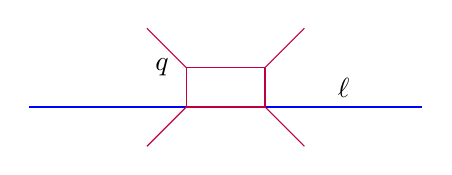
\begin{tikzpicture}[scale=.5]

\draw[thick, blue] (-5,0) to (5,0);
\node [above] at (3,0) {$\ell$};

\draw[purple] (-2,-1) to (-1,0);
%\draw[purple, dotted] (-2,-1) to (-2.1,-1.1);

\draw[purple] (-1,0) to (1,0);
\draw[purple] (1,0) to (2,-1);
\draw[purple] (-1,0) to (-1,1);
\draw[purple] (-1,1) to (-2,2);
\draw[purple] (-1,1) to (1,1);
\draw[purple] (1,1) to (2,2);
\draw[purple] (1,1) to (1,0);

\node [left] at (-1.2,1) {$q$};
\end{tikzpicture}
\caption{Intersection along a bounded edge}
\label{BoundedHorizontal}
\end{figure}

\end{example}

Another way of seeing that the tangency point must be at the middle of the segment is via modifications. 
%\subsection{Intersection at a vertex of the line and an edge of the curve} 


\section{Results}
\begin{thm}\label{thm:tropdual}
For $X$ sufficiently generic \yoav{(is tropically smooth generic enough?)}, we have
\[
\trop(X^*)=(\trop(X))^*.
\]
\end{thm}
\begin{proof}
Since tangents tropicalize to tropical tangents, we have an inclusion $\trop(X^*)\subseteq(\trop(X))^*$ as polyhedral complexes. The other inclusion follows from the fact that tropical tangents lift. The fact that the weights agree is an intersection calculation \nathan{\ldots}. 
\end{proof}
\nathan{We need to be careful in our arguments to make sure we are only discussing tangents at smooth points!}



We may use Theorem \ref{thm:tropdual} to describe the behaviour of the Newton polytope $\Delta_X$ of $X$ under taking projective duals:
\begin{thm}\label{thm:newton}
Let $X\subset \PP^2$ be an irreducible plane curve sufficiently generic with respect to $\Delta_X$. Let the edge vectors of $\Delta_X$ be $e_1,e_2,\ldots,e_m$ in counterclockwise orientation, omitting all edges parallel to $(1,0)$, $(0,-1)$, and $(-1,1)$. For each of these latter three vectors $w$, let $s_w$ be the sum of the edge vectors parallel to $w$, and set $c_w=s_w/w$. 

Then the edge vectors of $\Delta_{X^*}$ are exactly  $-e_m,\ldots,-e_1$, along with $(\vol (\Delta_X)-c_w)\cdot w$. 
Here, $\vol$ denotes the normalized lattice volume.
\end{thm}
\begin{proof}
The edges of $\Delta_{X^*}$ are determined by the unbounded edges of $C^*=\trop(X^*)=(\trop(X))^*$. 
Let $T$ be the regular unimodular triangulation of $\Delta_X$ induced by the valuations of the coefficients of $f$. The tropical curve $\trop(X)$ is dual to this triangulation.


We use the explicit description of $C^*$ to see: for $u\in \{(1,0),(0,1),(-1,-1)\}$, the number of rays in direction $u$ (counted with multiplicity) is given by $2\cdot a_u+b_u$ where $a_u$ is the number of edges of $C$ parallel to $u$ excluding rays in direction $-u$, and $b_u$ is the number of vertices of $C$ not having an edge parallel to $u$.
We can reinterpret $2\cdot a_u$ as the number of vertices of $C$ having an edge parallel to $u$, plus the number of rays of $C$ in direction $u$, less the number of rays of $C$ in direction $-u$.
Let $T'$ consist of those triangles in $T$ with an edge orthogonal to $u$, and $T''=T\setminus T'$. Then $\#T''=b_u$, and $\#T'$ is the number of vertices of $C$ having an edge parallel to $u$.

It is easily verified that 
\[2a_u+b_u=\#T'+\#T''-c_w\]
where $w$ is orthogonal to $u$ and $\det (u,w)=1$. Since $\vol(\Delta_X)=\#T=\#T'+\#T''$, the formula for the length of the edge of $\Delta_{X^*}$ in direction $w$ follows.

For $u\notin\{(1,0),(0,1),(-1,-1)\}$, 
the number of rays in direction $u$ (counted with multiplicity) is given by the number of rays of $C$ in direction $-u$. The edge length formula for edges orthogonal to $u$ now easily follows.
\end{proof}

Let $\Delta$ be the convex hull of $(0,0)$, $(1,0)$, and $(0,1)$.

\begin{ex}
If $X$ is a generic plane curve of degree $d$, its Newton polytope is $d\cdot \Delta$, and it is sufficiently generic with respect to its Newton polytope. By the above, the Newton polytope $\Delta_{X^*}$ has edges in directions $w=(1,0)$, $(-1,1)$, and $(0,-1)$, each of length
\[
\vol(\Delta_X)-c_w=d^2-d.
\]
Hence, $\Delta_{X^*}=(d^2-d)\cdot \Delta$, and we recover the classical fact that a generic degree $d$ plane curve has dual of degree $d(d-1)$.
\end{ex}

\begin{ex}
Let $X$ be a generic plane curve of degree $d$ with an isolated nodal or cuspidal singularity at the origin. After changing coordinates, we can assume that its Newton polytope is
\[
\conv \{(2,0),(d,0),(0,d),(0,2)\}
\] 
in the nodal case or 
\[
\conv \{(3,0),(d,0),(0,d),(0,2)\}
\] 
in the cuspidal case. 
By the above theorem, we obtain that  $\Delta_{X^*}$ has edges
\[
(d^2-d-2)(1,0),(d^2-d-2)(-1,1),(d^2-d-2)(0,-1)
\]
in the nodal case and
\[
(d^2-d-3)(1,0),(d^2-d-6)(-1,1),(-3,2)(d^2-d-4)(0,-1)
\]
in the cuspidal case.
Thus, in the nodal case, $\Delta_{X^*}=(d^2-d-2)\Delta$, and $X^*$ has degree $d(d-1)-2$. 
In the cuspidal case, the smallest dilate of $\Delta$ in which $\Delta_{X^*}$ fits is $(d^2-d-3)\Delta$, so 
$X^*$ has degree $d(d-1)-1$.

Combining this with the fact that the decrease to degree of $X^*$ from each singularity of $X$ is local \nathan{??}, we recover Pl\"ucker's classical formula that every node of $X$ lowers the degree of the dual curve by $2$, and every cusp by $3$.
\end{ex}

We can describe more generally how singularities contribute to the decrease in degree of the dual curve:


\begin{lemma}
	\label{Lemma:dual_degree}
Let $X$ be an irreducible projective plane curve of degree $d$ with which is generic with respect to its Newton polytope, and with  $Q=(0:0:1)$ the only singular point.
Let $A$ be the area of the complement of the Newton polyhedron of $X$ at $Q$, $\bernd{\nu}$ the multiplicity of $Q$ in $C$, and $\tau$ the intersection multiplicity of the union of the coordinate axes with $X$ at $Q$. 
Then the degree of $X^*$ is $d^2-d-\delta$, where 
\[
\delta=A+\bernd{\nu}-\tau
\]
\end{lemma}

\bernd{Note that $ \delta = 0 $ if $ \nu = 1 $.}

\begin{proof}
Consider the Newton polytope $\Delta_X$ of $X$; it has vertices $(d,0)$, $(0,d)$, and 
\[(a_1,b_1),\ldots, (a_m,b_m), \qquad 0=a_1<a_2<\ldots <a_m;\ b_1>b_2>\ldots>b_m=0.
\]
Let $k$ be the index such that $(b_{i+1}-b_i)/(a_{i+1}-a_i)$ is smaller than $-1$ if and only if $i<k$.  Note that the area $A$ mentioned above is simply $d^2$ less the area of $\Delta_X$. Using our description of $\Delta_{X^*}$ from Theorem \ref{thm:newton}, it is apparent that $(0,0)$ is a vertex of $\Delta_{X^*}$. It is then not difficult to verify that the degree of $X^*$ is given by the length of the edge in direction $(1,0)$ of $\Delta_{X^*}$, plus $b_1-b_k+a_1-a_k$.
But this is the same as 
\begin{align*}
d^2-A-(d-a_m)+(b_1-b_k+a_1-a_k)\\
=d^2-d-(A-a_m-b_1+a_k+b_k),
\end{align*}
and $a_k+b_k$ is the multiplicity of $Q$ in $X$, and $a_m+b_1$ is the intersection multiplicity at $Q$ of the union of the coordinate axes with $X$.
\end{proof}

Since each singularity of $X$ contributes independently to the lowering of the degree of $X^*$, we can use the above lemma to calculate the degree of $X^*$ for arbitrary $X$, just so long as for every singularity $Q$ of $X$, under some change of coordinates, $X$ at $Q$ is generic with respect to its Newton polytope \nathan{Make this precise. Is this always the case? Compare with Noether's formula.}

\smallskip

\bernd{NEW:}
In order to make this more precise, we draw a connection with 
Teissier's generalized Pl\"ucker formula, \cite{LNM777} II.3.
In our situation this states the following 
(see also \cite{Teissier_Trieste} section 11):
Let $ X $ be a an arbitrary reduced projective plane curve of degree $ d $,
then the degree of $ X^* $ is 
$ d^* = d ( d - 1) - \sum\limits_{Q \in \mathrm{Sing}(X) } \Delta_{X,Q} $, where
$$
	\Delta_{X,Q} = \mu(X,Q) + \nu(X,Q) - 1 ,
$$
and $ \mu(X,Q) $ denotes the Milnor number of $ (X,Q) $ and 
$ \nu(X,Q) $ denotes the multiplicity of $ X $ at $ Q $. 

In Lemma \ref{Lemma:dual_degree}, we have seen that the diminution due to
the singularity $  $ is $ \delta_{X,Q} := \delta = A + \nu - \tau $ 
(neglecting the dependence on $ X $ and $ Q $ for simplicity)
if $ X $ is generic with respect to its Newton polytope.
The first condition that we need to impose on $ X $ is that it is {\em convenient}
(in French {\em commode} \cite{Kouchnirenko} 1.5 D\'efinition), 
i.e., its Newton polytope intersects every coordinate axis.


Locally at $ Q $, $ X $ is given by some formal series $ f = \sum\limits_{(i,j) \in \NN^2} a_{ij} x^i y^j $, where $ (x,y) $ are local coordinates.
We denote by $ \Delta_f $ the Newton polytope of $ f $. 
(Recall that $ \Delta_f $ is the convex hull of $ \{ (i,j) + \RR^2_{\geq 0} \mid a_{ij} \neq 0   \} $).
Denote by $ \Delta_f^c $ the union of the compact faces of $ \Delta_f $. 
The {\em Newton principal part} of $ f $ is the polynomial 
$ f_0 = \sum\limits_{(i,j) \in \Delta_f^c} a_{ij} x^i y^j $
defined by those monomials contributing to $ \Delta_f^c $
(\cite{Kouchnirenko} 1.6 D\'efinition I).
Since $ X $ is convenient, the same is true for $ f $.
Note that 
$$ 
	\delta_{X,x} - (\nu(X,x) - 1) = A - \tau + 1 
$$ 
is exactly the Newton number of $ f $
(see \cite{Kouchnirenko} D\'efinition 1.7 and 1.8).
Kouchnirenko proved that the Newton number of a formal power series $ f $ 
is a lower bound for its Milnor number $ \mu (f) = \mu (X,x) $,
see \cite{Kouchnirenko} 1.10 Th\'eor{\`e}me I.
Furthermore, he gave a citerion when both coincide:
we have
$$
	 A - \tau + 1 = \mu (f)
	 \ \ \ \ \ \ 
	 (\mbox{and thus }
	 \Delta_{X,x} = \delta_{X,x})
$$
if the Newton principal part of $ f $ is {\em non-degenerate}, 
i.e.,
for each closed face $ \Delta $ of $ \Delta^c_f $ the polynomials 
$ (x \frac{\partial f}{\partial x})_\Delta, (y \frac{\partial f}{\partial y})_\Delta $ 
do not have a common zero in $ ( \CC \setminus \{ 0 \} )^2 $,
% (In general, in $ ( \overline K \setminus \{ 0\} )^n $ if there are $ n $ coordinates and $ K $ is the base field).
(\cite{Kouchnirenko} D\'efinition 1.19).
Here, $ g_\Delta := \sum_{(i,j) \in \Delta} b_{ij} x^i y^j $ denotes the terms 
contributing to $ \Delta $, for some formal series 
$ g = \sum_{(i,j) \in \NN^2} b_{ij} x^i y^j $. 

\begin{rem} 
In fact, Teissier's formula is valid for $ n $-dimensional complex
hypersurfaces $ X $ with at most isolated singularities, $ n \in \NN$.
Then the degree of $ X^* $ is given by
$$	
	d^* = d (d-1)^n - \sum_{Q \in \mathrm{Sing} (X)} ( \mu^{(n)} (X,Q) + \mu^{(n+1)}(X,Q)) ,
$$
where $ \mu^{(n+1)}(X,Q) $ denotes the Milnor number of $ (X,Q) $ and
$ \mu^{(n)}(X,Q) $ denotes the Milnor number at $ Q $ of a general hyperplane
section of $ X $, \cite{LNM777} II.3.
%i.e., of $ X \cap H \subset H $ for a general hyperplane $ H $. 

By Kouchnirenko's result, we know that the Milnor number can be computed as
an alternating sum of $ k $-dimensional volumes of polyehdra  coming from the
Newton polyhedron. 
Thus $ \mu^{(n)} (X,Q) $ and $ \mu^{(n+1)}(X,Q) $ can be translated into terms 
coming from the Newton polyhedron. 

\bernd{As a consequence of Theorem \ref{thm:newton} we obtain that 
$ \Delta_{X^*} $ can be determined by Minkowski sums of certain edge vectors 
of $ \Delta_X $ once we know $ d^* $.
It is possible to make this procedure precise in the higher dimensional case.
Combining this with the above two results we can determine the dual Newton polyhedron
in any dimension. 
From this we can then deduce a tropical variety.
If Theorem \ref{thm:tropdual} holds in any dimension, this should be the dual 
of the tropical variety $ \trop (X) $.
}
\end{rem} 

%\section{Real tropical curves}
%A non-singular real tropical curve is a tropical curve together with a subset $T$ of its bounded edges called \emph{twisted edges} such that for all cycles $\gamma$ contained in $\Gamma$ we have:
%$$\sum_{e \in T} v_e \equiv (0, 0) \mod 2,$$
%where $v_e$ is the primitive integer direction of the edge $e$. 


\section{Nathan's Calculations on Lifting}
\subsection{Necessary conditions}
We now consider a hypersurface $X=V(f)\in\PP^n$ for $f=\sum_{u\in\A} c_u x^u$. Here $\A$ is a subset of $\ZZ^{n+1}$. Assume that $\trop(X)$ is smooth.
Notation: for any $q\in K$, $q=\overline q+q'$, where $\overline q$ is the lowest order term. We will always use $\HOT$ to denote higher order terms.

Fix a point $p=(p_0,\ldots,p_n)\in\trop(X)$. We are interested in all describing $\trop(H)$ for all hyperplanes $H$ tangent to $X$ at smooth points $x$ with $\trop(x)=p$. Let $p$ be contained in the interior of a $d$-cell $E$ of $\trop(X)$. Let $\A_{E}$ be the set of $n+1-d$ elements of $\A$ corresponding to $E$.
Then for any point $x$ with $\trop(x)\in E$, we have 
\[
f=\sum_{u\in\A_E} \overline{c}_u\overline{x}^u+\HOT.
\]
If $x\in X$, then the above sum must vanish.

The hyperplane tangent to $X$ at $x$ is (given in dual coordinates) $y=(f_{x_0},f_{x_1},\ldots,f_{x_n})$. We wish to understand $\trop(y)$. Now, note that we have
\[
x_if_{x_i}=\sum_{u\in\A_E} u_i\overline{c}_u\overline{x}^u+\HOT.
\]
Therefore, if the leading terms don't cancel each other, then $\trop(y_i)+p_i$ equals $u\cdot\trop{x} +\trop(c_u)$ for any $u\in\A_E$ (this doesn't depend on the choice of  $u\in\A_E$). Since $u\cdot\trop{x} + \trop(c_u)$ doesn't depend on $i$ and we work in projective coordinates, we shift all the coordinates by it, and conclude that $\trop(y_i)\leq -p_i$, with ``$<$'' if and only if 
\begin{equation}\label{eqn:df}
\sum_{u\in\A_E} u_i\overline{c}_u\overline{x}^u=0.
\end{equation}
\nathan{NEW STUFF}
We thus arrive at a necessary condition for the coordinates of $\trop(H)$: let $a_u=\overline{c_u x^u}$, and let $I$ be the set of indices for which $\trop(y_i)<p_i$, with complement $I^c$.
For any $u$, let $e_u$ be the vector in $\ZZ^{\A_E}$ with entry $1$ at position $u$ and $0$ elsewhere.
Then the $(|I|+1)\times |\A_E|$-matrix 
\begin{equation}\label{eqn:s1}
\left(\begin{array}{c}
1\\
u_{i}
\end{array}\right)_{i\in I,u\in \A_E}
\end{equation}
must satisfy
\begin{equation}\label{eqn:s2}
\left(\begin{array}{c}
1\\
u_{i}
\end{array}\right)\cdot (a_u)=0
\end{equation}
and for all $i\in I^c$,
\begin{equation}\label{eqn:s3}
(u_i)\cdot (a_u)\neq 0.
\end{equation}
Note furthermore the requirement that for all $u$, $a_u\neq 0$.

Such a solution $(a_u)$ to \eqref{eqn:s2} and \eqref{eqn:s3} exists only if
\begin{enumerate}
\item The rowspan of the matrix \eqref{eqn:s1} does not contain the vector $e_u$ for any $u$.
  \item The rowspan of the matrix \eqref{eqn:s1} does not contain any vector $(u_i)$ for fixed $i\in I^c$.
\end{enumerate}
These conditions can be interpreted as follows.
\begin{enumerate}
\item Any direction $v$ emanating from $E$ which is contained in $\langle e_i\rangle _{i\in I}$ is already contained in $\langle E-E\rangle$.
\item For any $j\in I^c$,
  \[
\langle E-E\rangle \cap \langle e_i\rangle _{i\in I}
=\langle E-E\rangle \cap \langle e_j,e_i\rangle _{i\in I}.
  \]
  \end{enumerate}

Now, given a solution to \eqref{eqn:s2} and \eqref{eqn:s3}, we need to actually show that it lifts to higher order (and to count multiplicity). The idea is to perform row operations to \eqref{eqn:s1} until it is in reduced row echelon form. The new equations (linear combinations of the $f, x_if_{x_i}$) should now have tropicalizations which intersect transversely at the desired point.
If this matrix doesn't have full rank, then higher order terms of the $x_if_{x_i}$ come into play.



\nathan{BACK TO OLD STUFF}
Firstly, consider the case that $u_i=0$ for all $u\in \A_E$. Then $E$ is unbounded in direction $-e_i$. In direction $e_i$, it borders on a $d-1$ cell $E'$; this corresponds to an additional element $v\in \A\setminus \A_E$ with $v_i\neq 0$. By smoothness, it must be that $v_i=1$. 
When differentiating with respect to $x_i$, all the monomials coming from $\A_E$ vanish, and the leading term becomes $v_i\overline{c}_v \overline{x}^v$. We claim that $\trop{y_i}=-p_i' + u\cdot\trop(x) + \trop(c_u)$, where $p'$ is the unique point of $E'$ whose coordinates coincide with the coordinates of  $p$ except for the $i$-th coordinate.  In other words, the $i$-th coordinate of the tropical dual plane is just $p_i'$.
Indeed, for $x'$ tropicalizing to $p'$, the terms $v\cdot\trop(x') + \trop(c_v)$  and $u\cdot\trop(x') + \trop(c_u)$ coincide. Since $\trop(x') = \trop(x) + e_i(p'_i-p_i)$, we get
\[
[\trop(x) + e_i(p_i'-p_i)]\cdot u + \trop(c_u) = [\trop(x) + e_i(p_i'-p_i)]\cdot v + \trop(c_v).
\]
It follows that 
\[
(u-v)\cdot \trop(x) = \trop(c_v) - \trop(c_u) + (p_i'-p_i) e_i\cdot (v-u).
\]
Using the face that $e_i\cdot (v-u) =1$ the result follows.


%Then 
%\[
%\overline{x}_if_{x_i}=v_i+=\overline{c}_v\overline{x}^v+\sum_{u\in\A_E} u_i\overline{c}_u\overline{x}^u+\HOT
%=\overline{c}_v\overline{x}^v+\HOT.
%\]
%Hence, $\trop(y_i)=-p_i'$, where $p_i$ is the $i$th coordinate of $E'$. 
\nathan{This is not quite correct}. \yoav{why not?}


Secondly, consider the case that $u_i=0$ for all but one $u\in \A_E$. Then Equation \eqref{eqn:df} is impossible to satisfy, so we conclude $\trop(y_i)=-p_i$. 

Finally, consider some set of indices $I\subset [0,n]$ such that for $i\in I$, at least two $u\in \A_E$ satisfy $u_i\neq 0$. If $|I|\geq n-d$, we cannot have $\trop(y_i)<-p_i$ for all $i\in I$. Indeed, to do so would require that the  $(n+1-d)\times (n+1-d)$ matrix with columns 
\[
\left(\begin{array}{c}
1\\
u_{i_1}\\
\vdots\\
u_{i_{n-d}}
\end{array}\right)
\]
indexed by $u\in\A_E$ be singular. Here, $\{i_1,\ldots,i_{n-d}\}\subset I$. But since the vectors $u\in \A_E$ form the vertices of a simplex, this matrix is invertible unless some $e_{i_j}$ is orthogonal to this simplex, that is, $E$ contains a segment in direction $e_{i_j}$. \nathan{Flesh this out.}

Thus, we have shown the following: \nathan{fill in details}
\begin{prop}
The tropical dual hypersurface $\trop(X^*)$ is contained in the following polyhedral complex:
\[
\bigcup_{E,I}  -(E+L_I)
\]
where $E$ is taken to be any cell of $\trop(X)$ which is bounded in all directions $e_0,e_1,\ldots,e_n$, $I$ is a subset of $[0,n]$ of size \nathan{at most??} $n-\dim E -1$ such that $E-\RR_{\geq 0}e_i$ is not \nathan{a cell?} in $\trop(X)$, and $L_I=\RR_{\geq 0}\cdot \{e_i\ |\ i\in I\}$.   
\end{prop}

\subsection{Sufficient conditions}
%\bibliographystyle{amsalpha}
%\renewcommand{\MR}[1]{\relax}
%\bibliography{fano-split}

We do several ``easy'' cases to start:
\subsubsection{Non-shifted points on $\trop(X)$}\label{sec:nonshift}

Suppose that $p\in E$. We show (under additional assumptions) that $-p$ is in $\trop(X^*)$.
Let $g_i=f_{x_i}-y_i$
We are looking for a solution $x_i,y_i$ to 
\[f=g_0=\ldots=g_n=0\]
such that $\overline{y}_i=-p_i$. From the above, we see that this last condition equivalent to requiring that 
\begin{equation*}
\sum_{u\in\A_E} u_i\overline{c}_u\overline{x}^u\neq0.
\end{equation*}
Setting $a_u=\overline{c}_u\overline{x}^u$, this means that we need to find $a_u$ such that 
\begin{align*}
\sum a_u=0\\
\sum u_i a_u \neq 0\ \quad \forall i.
\end{align*}
If for fixed $i$ not all $u_i$ are the same value, then choosing $a_u$ generic will satisfy the above. If $\dim E=0$, then we can recover the $\overline{x}_i$ from the $a_u$, otherwise, we are allowed to make some additional choices. Note that once we fix the $\overline{x}_i$, we have also fixed the $\overline{y}_i$.

In fact, we can now choose $x_1',\ldots,x_n'$ arbitrarily, leaving $x_0$ and $y_0,\ldots,y_n$ as unknowns. To apply Hensel's Lemma to the system
\[f=g_0=\ldots=g_n=0,\]
we need to verify that the determinant of 
\[
\left(
\begin{array}{c c c c}
\frac{\partial f}{\partial x_0} &  \frac{\partial f}{\partial b_0} & \cdots &\frac{\partial f}{\partial b_n}\\
\frac{\partial g_0}{\partial x_0} &  \frac{\partial g_0}{\partial b_0} & \cdots &\frac{\partial g_0}{\partial b_n}\\
\vdots&&&\vdots\\
\frac{\partial g_n}{\partial x_0} &  \frac{\partial g_n}{\partial b_0} & \cdots &\frac{\partial g_n}{\partial b_n}\\
\end{array}
\right)
\]
has valuation \nathan{??}. But taking lowest order terms of each entry, we obtain the matrix 
\[
\left(
\begin{array}{c c c c}
\overline{y}_0 & 0\\
0 & I_{n+1}
\end{array}
\right)
\]
which has the desired property.

\nathan{If for fixed $i$ all $u_i$ are equal, we \emph{cannot} lift. This is equivalent to $E$ containing direction $e_i$. Conversely, as long as this is not the case, we are OK.}

\begin{rem}
This shows in particular that if $p$ is a vertex of $\trop(X)$, then $-p$ is in $\trop(X^*)$.
\end{rem}

\subsubsection{Interior vertex of $\trop(X)$}
Suppose now that $v$ is an ``interior'' vertex of $\trop(X)$. We wish to show that for $\lambda_2,\ldots,\lambda_{n}>0$, $-p-\sum \lambda_i e_i\in\trop(X^*)$. We again look for a solution to 
\[f=g_0=\ldots=g_n=0.\]
To solve the lowest order part of this, we need that
\begin{align*}
\sum a_u=0\\
\sum u_i a_u \neq  0\ \quad \forall i\leq 1.\\
\sum u_i a_u = 0\ \quad \forall i>1.
\end{align*}
Since the matrix with top row consisting of $1$, and the remaining entries $(u_i)$ (columns indexed by $u$, rows by $i$) with $i>1$ has rank less than $n+1$, this system has a non-zero solution: note that the two $\neq 0$ conditions must follow from the $=0$ conditions by a rank argument.
 \nathan{but we need all entries non-zero -- can we do that?}.

\nathan{In general, the answer is no. For example if $n=2$, then we have a problem exactly when the vertex $v$ has a ray eminating in the $e_2$ direction. However, if some $a_u=0$, we just throw those $u$ out and move to the interior of a larger cell in $\trop(X)$. We should be able to adapt the other arguments to this situation.}


The $a_u$ determine the $\overline{x}_i$, as well as the $\overline{y}_0,\overline{y}_1$. We now fix arbitrary $y_2,\ldots,y_n$, and treat $y_0,y_1,x_0,x_2,\ldots,x_n$ as variables.

we need to verify that the determinant of 
\[
\left(
\begin{array}{c c c c c c}
\frac{\partial f}{\partial y_0} &  \frac{\partial f}{\partial y_1} &  \frac{\partial f}{\partial x_0}  & \frac{\partial f}{\partial x_2} &\cdots &\frac{\partial f}{\partial x_n}\\
\frac{\partial g_0}{\partial y_0} &  \frac{\partial g_0}{\partial y_1} &  \frac{\partial g_0}{\partial x_0}  & \frac{\partial g_0}{\partial x_2} &\cdots &\frac{\partial g_0}{\partial x_n}\\

\vdots&&&&&\vdots\\
\frac{\partial g_n}{\partial y_0} &  \frac{\partial g_n}{\partial y_1} &  \frac{\partial g_n}{\partial x_0}  & \frac{\partial g_n}{\partial x_2} &\cdots &\frac{\partial g_n}{\partial x_n}\\
\end{array}
\right)
\]
has valuation \nathan{??}. But taking ``lowest order'' terms of each entry, we obtain the matrix 
\[
\left(
\begin{array}{c c c c c c}
0 &  0 &  \overline{y}_0  & 0 &\cdots & 0\\
1 &  0 &  \frac{\partial g_0}{\partial x_0}  & \frac{\partial g_0}{\partial x_2} &\cdots &\frac{\partial g_0}{\partial x_n}\\
0 &  1 &  \frac{\partial g_1}{\partial x_0}  & \frac{\partial g_1}{\partial x_2} &\cdots &\frac{\partial g_1}{\partial x_n}\\

\vdots&&&&&\vdots\\
0 &  0 &  \frac{\partial g_n}{\partial x_0}  & \frac{\partial g_n}{\partial x_2} &\cdots &\frac{\partial g_n}{\partial x_n}\\
\end{array}
\right)
\]
Hence, we need to show that the determinant of 
\[
\left(
\begin{array}{  c c c}
\frac{\partial g_2}{\partial x_2} &\cdots &\frac{\partial g_2}{\partial x_n}\\

\vdots&&\vdots\\
 \frac{\partial g_n}{\partial x_2} &\cdots &\frac{\partial g_n}{\partial x_n}\\
\end{array}
\right)
\]
has the correct valuation.
The lowest order terms we are interested in will be (up to scalars)
\[
\left(
\begin{array}{  c c c}
x_2x_2\frac{\partial^2 f}{\partial x_2\partial x_2} &\cdots &x_2x_n\frac{\partial^2 f}{\partial x_2\partial x_n}\\

\vdots&&\vdots\\
x_nx_2\frac{\partial^2 f}{\partial x_n\partial x_2} &\cdots &x_nx_n\frac{\partial^2 f}{\partial x_n\partial x_n}\\
\end{array}
\right)
\]

Note that
\[
x_ix_j\frac{\partial^2 f}{\partial x_i\partial x_j}=
\sum_u u_iu_j a_u+\HOT  
\]
(for $i=j$ we are using $\sum u_ia_u=0$).
So we are left showing that the $a_u$ don't satisfy a certain polynomial equation.


I have no idea how to do this in general, but if $n=2$, we just need to show that 
\[
\sum_u u_2^2a_u\neq 0.
\]
In other words, if the $\A_E=\{u,v,w\}$ we need that the matrix 
\[
\left(\begin{array}{c c c}
1&1&1\\
u_2&v_2&w_2\\
u_2^2& v_2^2& w_2^2
\end{array}\right)
\]
is non-singular. But this is a Vandermonde matrix, with determinant $\pm (u_2-v_2)(u_2-w_2)(v_2-w_2)$. We had already excluded the case that one of these factors vanishes, so we do get the desired lifting!!

\subsubsection{Interior edge of $\trop(X)$ in curve case}
If the edge $E$ is not in some direction $e_i$, then we are already done by the obstructions and the lifting of \S\ref{sec:nonshift}
Suppose instead that $E$ is in WLOG direction $e_2$, and take $p\in E$. 

We wish to show that for $\lambda_2>0$, $-p- \lambda_2 e_2\in\trop(X^*)$. We again look for a solution to 
\[f=g_0=\ldots=g_2=0.\]
To solve the lowest order part of this, we need that
\begin{align*}
\sum a_u=0\\
\sum u_i a_u = 0\ \quad i=2.
\sum u_i a_u \neq  0\ \quad i=0,1.\\
\end{align*}
Here the sums are just over two elements, say $u$ and $v$.  But since $u_2=v_2$ by assumption, we can take any $a_v=-a_u\neq 0$ as a solution. 

The $a_u$ partially determine the $\overline{x}_i$, we are left with one-parameter worth of choice. This then also determines the $\overline{y}_0,\overline{y}_1$. We now fix arbitrary $y_2$, and treat $y_0,y_1,x_0,x_2$ as variables.

As before we will arrive at a determinant
\[
\left(
\begin{array}{c c c c }
0 &  0 &  \overline{y}_0  & 0 \\
1 &  0 &  \frac{\partial g_0}{\partial x_0}  & \frac{\partial g_0}{\partial x_2} \\
0 &  1 &  \frac{\partial g_1}{\partial x_0}  & \frac{\partial g_1}{\partial x_2} \\

0 &  0 &  \frac{\partial g_2}{\partial x_0}  & \frac{\partial g_2}{\partial x_2} \\
\end{array}
\right)
\]
The only relevant term for us is thus 
\[\frac{\partial g_2}{\partial x_2} 
=u_2(u_2-1)a_u+v_2(v_2-1)a_v+\HOT
=u_2^2a_u+v_2^2a_v+\HOT
\]
\nathan{Unfortunately this vanishes :(}

Better strategy: choose arbitrary $x_2$, and use $x_1$ as a variable instead. Then we get:
\[
\left(
\begin{array}{c c c c }
0 &  0 &  \overline{y}_0  & \overline{y}_1 \\
1 &  0 &  \frac{\partial g_0}{\partial x_0}  & \frac{\partial g_0}{\partial x_1} \\
0 &  1 &  \frac{\partial g_1}{\partial x_0}  & \frac{\partial g_1}{\partial x_1} \\

0 &  0 &  \frac{\partial g_2}{\partial x_0}  & \frac{\partial g_2}{\partial x_1} \\
\end{array}
\right)
\]
and we are left looking at
\[
\left(
\begin{array}{ c c }
  \overline{y}_0  & \overline{y}_1 \\

  \frac{\partial g_2}{\partial x_0}  & \frac{\partial g_2}{\partial x_1} \\
\end{array}
\right)
=
\left(
\begin{array}{ c c }
  \overline{y}_0  & \overline{y}_1 \\
u_0u_2a_u+v_0v_2a_v&
u_1u_2a_u+v_1v_2a_v
\end{array}
\right).
\]
Since $u_2=v_2$, we can rescale the second row to get
\[
\left(
\begin{array}{ c c }
  \overline{y}_0  & \overline{y}_1 \\
u_0a_u+v_0a_v&
u_1a_u+v_1a_v
\end{array}
\right).
\]
But this matrix is singular. \nathan{AARRRGGG}



\subsection{Lifting revisited}
Here I consider the case of curves and lifting tangents to a point on a ``horizontal'' edge. Essentially, this is my attempt to understand Yoav's calculation from a different perspective.

Notation: $X=V(f)$ for $f\sum_{u\in \A} c_ux^u$. I assume that we are working over Puiseux series, say with parameter $t$. By $t\mapsto t^{1/m}$, I can (and will) assume that all exponents are integral. If $s$ is such a series, then $s[k]$ denotes the coefficient of $t^k$.

Now, fix a point $p\in \trop(X)$ contained in the interior of a bounded horizontal edge.
By rescaling and translating, we can actually assume that $p=0$.
The lowest order terms of $f$ are achieved exactly by some $c_vx^v$ and $c_wx^w$ with $v_1=w_1=r$. As we've seen above, the only possible tangents to a point tropicalizing to $p$ are those tropicalizing to $-p-\lambda e_1$ for $\lambda >0$.

Now, the zeroeth order system we need to solve is:
\begin{align*}
	f(x)[0]=x_1^r[0]\left(c_v[0]x_0^{v_0}[0]x_2^{v_2}[0]+c_w[0]x_0^{w_0}[0]x_2^{w_2}[0]\right)=0\\
	rf(x)[0]-x_1[0]\frac{\partial f}{\partial x_1}(x)[0]=0\\
	x_0[0]\frac{\partial f}{\partial x_0}(x)[0]\neq 0\\
	x_2[0]\frac{\partial f}{\partial x_2}(x)[0]\neq 0\\
\end{align*}
The second equation is always satisfied, as are the third and fourth. The first equation we can solve by appropriate choices of $x_0[0]$ and $x_2[0]$.

Now, $rf(x)-x_1\frac{\partial f}{\partial x_1}(x)$ is automatically identically zero up to the order $m$ where there is $c_u$, $u\in \A$ with $u_1\neq r$ with the order of $c_u$ equal to $m$. Let's call $m$ the \emph{critical order}. Set $\A'$ to be those $u\in \A$ with $c_u$ of critical order and $u_1\neq r$.

To lift our zeroeth order solution below the critical order, we only need to solve $f(x)[1]=f(x)[2]=\ldots=f(x)[m-1]=0$. At each step, we are faced with an equation of the form 
\begin{align*}
	f(x)[i]=x_1^r[0](v_0c_v[0]x_0^{v_0-1}[0]x_2^{v_2}[0]x_0[i]+w_0c_w[0]x_0^{w_0-1}[0]x_2^{w_2}[0]x_0[i]+\\
+v_2c_v[0]x_0^{v_0}[0]x_2^{v_2-1}[0]x_2[i]+w_2c_w[0]x_0^{w_0}[0]x_2^{w_2-1}[0]x_2[i])+C_i\\
=0
\end{align*}
where $C_i$ only depends on $x_0,x_2$ up to order $i-1$. We see that we are faced with solving an inhomogeneous linear equation in $x_0[i]$ and $x_2[i]$ with coefficients respectively 
\begin{align*}
	x_0^{-1}(v_0c_v[0]x^v[0]+w_0c_w[0]x^{w}[0])\\
	x_2^{-1}(v_2c_v[0]x^v[0]+w_2c_w[0]x^{w}[0])
\end{align*}
neither of which is zero by the zeroeth order condition. Note of course that these coefficients are just the lowest order parts of $\frac{\partial{f}}{\partial x_0}$ and $\frac{\partial{f}}{\partial x_0}$.
This means that we can lift to the critical order, and do so with arbitrary choices for e.g. the $x_0[i]$.

Now, we get to the critical order. {\bf First case}: $\A'$ contains only a single element. Then the $m$th order part of 
\[rf(x)-x_1\frac{\partial f}{\partial x_1}(x)\]
is a single monomial, hence cannot vanish. So the \emph{only} tangent we get for the point $p$ is the tangent $-p-me_1$. Note that this is actually the generic case: a generic point $p$ in an edge will land in this case (if we have chosen $X$ sufficiently generic so that all hyperplanes arising from comparing weights are distinct). This tangent actually does lift: we just need to continue lifting the equation $f(x)[i]=0$ for $i\geq m$. This has the same form as above, except that the constants $C_i$ will also depend on $x_1[j]$ for $j\leq i-m$.

This now takes us to the {\bf second case}: $\A'$ contains multiple elements.
Then 
\begin{align*}rf(x)-x_1\frac{\partial f}{\partial x_1}(x)=
	\sum_{u\in \A'}c_u[m]x^u(r-u_1)[0]+\HOT\\
\end{align*}
Now, by imposing the condition that $c_u[m]$ are sufficiently generic, we can achieve that the left hand side, as a polynomial in $x_1[0]$, has degree $d>0$, that is, some higher degree term doesn't cancel. Hence, we can either choose $x_1[0]$ such that this equation doesn't vanish (in which case we obtain the tangent $-p-me_i$ exactly as above), or we can impose vanishing; this gives $d$ choices for $x_1[0]$, counted with multiplicity.
\nathan{Details missing here. It is essential that the left hand side as a polynomial in $x_1[0]$ has at least two terms. This can be achieved in the smooth case: $\A'$ must contains elements ``on both sides'' of $u,v$.}


We now need to continue lifting to even higher order. At each step,  for $rf(x)-x_1\frac{\partial f}{\partial x_1}(x)$ we are faced with an equation of the form
\begin{align*}
	0=	\sum_{u\in \A'}c_u[m]x^u(u_1r-u_1^{2})[0]x_1^{-1}[0]x_1[i]+D_i\\
\end{align*}
where $D_i$ is a constant depending on lower order terms in $x_0x_1,x_2$. This is an inhomogeneous linear equation in $x_1[i]$. We can again demand that the $c_u[m]$ are sufficiently generic so that the coefficient 
\[
	\sum_{u\in \A'}c_u[m]x^u(u_1r-u_1^{2})[0]x_1^{-1}[0]x_1[i]
\]

for $x_1[i]$ is non-zero. 

What do we conclude? At each step of lifting for $i>m$, after fixing $x_0$, we have a unique solution  to $f=rf(x)-x_1\frac{\partial f}{\partial x_1}(x)=0$. Of course, at any point we wish, we can choose to not satisfy the latter equation. Thus, we obtain all tangents of the form $-p-ie_1$ for $i\geq m$. Note that for such a tangent, there are $d$ possible choices for $x_1[0]$, after fixing $x_0[0]$. This is presumably the multiplicity of this ray of the dual curve. \nathan{I have good reason to believe that in the smooth case we always have $d=2$. In fact, in that case $\A'$ (I believe) will consist of exactly the two monomials corresonding to the two vertices of the edge in which $p$ is located. This will force $p$ to be the midpoint, as previously stated by Yoav and Kristin.}


\begin{thebibliography}{bla}	

	\bibitem{BrugalleLopez} E.~Brugall\'e and L.~L\'opez de Medrano 
	\newblock {Inflection points of real and tropical plane curves} 
	\newblock{ https://arxiv.org/pdf/1102.2478v4.pdf }
		
	\bibitem{Kouchnirenko}
	A.~G.~Kouchnirenko,
	\newblock {Poly{\`e}dres de Newton et nombres de Milnor},
	\newblock {\em Invent. Math} {\bf 32} (1976), 1--31.
	
	\bibitem{LNM777}
	B.~Teissier,
	\newblock {R\'esolution simultan\'ee, I et II},
	\newblock in {\em S\'eminaire sur les singularit\'es des surfaces}, 71--146, Palaiseau 1976-77, Demazure, Pinkham, Teissier, Editors, Springer Lecture Notes in Math., No 777.
	
	\bibitem{Teissier_Trieste}
	B.~Teissier,
	\newblock {Complex curve singularities: a biased introduction},
	\newblock in {Singularities in geometry and topology},  825--887, World Sci. Publ., Hackensack, NJ, 2007. 
		
\end{thebibliography}
\end{document}
